% Created 2026-11-08 Sun 12:20
% Intended LaTeX compiler: pdflatex
\documentclass[11pt]{article}

\usepackage[utf8]{inputenc}
\usepackage[T1]{fontenc}
\usepackage{graphicx}
\usepackage{longtable}
\usepackage{wrapfig}
\usepackage{rotating}
\usepackage[normalem]{ulem}
\usepackage{amsmath}
\usepackage{amssymb}
\usepackage{capt-of}
\usepackage{hyperref}
\date{\today}
\title{}
\hypersetup{
 pdfauthor={},
 pdftitle={},
 pdfkeywords={},
 pdfsubject={},
 pdfcreator={},
 pdflang={English}}

% Setup for code blocks [1/2]

\usepackage{fvextra}

\fvset{%
  commandchars=\\\{\},
  highlightcolor=white!95!black!80!blue,
  breaklines=true,
  breaksymbol=\color{white!60!black}\tiny\ensuremath{\hookrightarrow}}

% Make line numbers smaller and grey.
\renewcommand\theFancyVerbLine{\footnotesize\color{black!40!white}\arabic{FancyVerbLine}}

\usepackage{xcolor}

% In case engrave-faces-latex-gen-preamble has not been run.
\providecolor{EfD}{HTML}{f7f7f7}
\providecolor{EFD}{HTML}{28292e}

% Define a Code environment to prettily wrap the fontified code.
\usepackage[breakable,xparse]{tcolorbox}
\DeclareTColorBox[]{Code}{o}%
{colback=EfD!98!EFD, colframe=EfD!95!EFD,
  fontupper=\footnotesize\setlength{\fboxsep}{0pt},
  colupper=EFD,
  IfNoValueTF={#1}%
  {boxsep=2pt, arc=2.5pt, outer arc=2.5pt,
    boxrule=0.5pt, left=2pt}%
  {boxsep=2.5pt, arc=0pt, outer arc=0pt,
    boxrule=0pt, leftrule=1.5pt, left=0.5pt},
  right=2pt, top=1pt, bottom=0.5pt,
  breakable}

% Support listings with captions
\usepackage{float}
\floatstyle{plain}
\newfloat{listing}{htbp}{lst}
\newcommand{\listingsname}{Listing}
\floatname{listing}{\listingsname}
\newcommand{\listoflistingsname}{List of Listings}
\providecommand{\listoflistings}{\listof{listing}{\listoflistingsname}}


% Setup for code blocks [2/2]: syntax highlighting colors

\newcommand\efstrut{\vrule height 2.1ex depth 0.8ex width 0pt}
\definecolor{EFD}{HTML}{000000}
\definecolor{EfD}{HTML}{ffffff}
\newcommand{\EFD}[1]{\textcolor{EFD}{#1}} % default
\definecolor{EFh}{HTML}{7f7f7f}
\newcommand{\EFh}[1]{\textcolor{EFh}{#1}} % shadow
\definecolor{EFsc}{HTML}{228b22}
\newcommand{\EFsc}[1]{\textcolor{EFsc}{\textbf{#1}}} % success
\definecolor{EFw}{HTML}{ff8e00}
\newcommand{\EFw}[1]{\textcolor{EFw}{\textbf{#1}}} % warning
\definecolor{EFe}{HTML}{ff0000}
\newcommand{\EFe}[1]{\textcolor{EFe}{\textbf{#1}}} % error
\definecolor{EFc}{HTML}{b22222}
\newcommand{\EFc}[1]{\textcolor{EFc}{#1}} % font-lock-comment-face
\definecolor{EFcd}{HTML}{b22222}
\newcommand{\EFcd}[1]{\textcolor{EFcd}{#1}} % font-lock-comment-delimiter-face
\definecolor{EFs}{HTML}{8b2252}
\newcommand{\EFs}[1]{\textcolor{EFs}{#1}} % font-lock-string-face
\definecolor{EFd}{HTML}{8b2252}
\newcommand{\EFd}[1]{\textcolor{EFd}{#1}} % font-lock-doc-face
\definecolor{EFm}{HTML}{008b8b}
\newcommand{\EFm}[1]{\textcolor{EFm}{#1}} % font-lock-doc-markup-face
\definecolor{EFk}{HTML}{9370db}
\newcommand{\EFk}[1]{\textcolor{EFk}{#1}} % font-lock-keyword-face
\definecolor{EFb}{HTML}{483d8b}
\newcommand{\EFb}[1]{\textcolor{EFb}{#1}} % font-lock-builtin-face
\definecolor{EFf}{HTML}{0000ff}
\newcommand{\EFf}[1]{\textcolor{EFf}{#1}} % font-lock-function-name-face
\definecolor{EFv}{HTML}{a0522d}
\newcommand{\EFv}[1]{\textcolor{EFv}{#1}} % font-lock-variable-name-face
\definecolor{EFt}{HTML}{228b22}
\newcommand{\EFt}[1]{\textcolor{EFt}{#1}} % font-lock-type-face
\definecolor{EFo}{HTML}{008b8b}
\newcommand{\EFo}[1]{\textcolor{EFo}{#1}} % font-lock-constant-face
\definecolor{EFwr}{HTML}{ff0000}
\newcommand{\EFwr}[1]{\textcolor{EFwr}{\textbf{#1}}} % font-lock-warning-face
\newcommand{\EFnc}[1]{#1} % font-lock-negation-char-face
\definecolor{EFpp}{HTML}{483d8b}
\newcommand{\EFpp}[1]{\textcolor{EFpp}{#1}} % font-lock-preprocessor-face
\newcommand{\EFrc}[1]{\textbf{#1}} % font-lock-regexp-grouping-construct
\newcommand{\EFrb}[1]{\textbf{#1}} % font-lock-regexp-grouping-backslash
\newcommand{\EFob}[1]{#1} % org-block
\definecolor{EFhn}{HTML}{008b8b}
\newcommand{\EFhn}[1]{\textcolor{EFhn}{#1}} % highlight-numbers-number
\definecolor{EFhq}{HTML}{9370db}
\newcommand{\EFhq}[1]{\textcolor{EFhq}{#1}} % highlight-quoted-quote
\definecolor{EFhs}{HTML}{008b8b}
\newcommand{\EFhs}[1]{\textcolor{EFhs}{#1}} % highlight-quoted-symbol
\definecolor{EFrda}{HTML}{707183}
\newcommand{\EFrda}[1]{\textcolor{EFrda}{#1}} % rainbow-delimiters-depth-1-face
\definecolor{EFrdb}{HTML}{7388d6}
\newcommand{\EFrdb}[1]{\textcolor{EFrdb}{#1}} % rainbow-delimiters-depth-2-face
\definecolor{EFrdc}{HTML}{909183}
\newcommand{\EFrdc}[1]{\textcolor{EFrdc}{#1}} % rainbow-delimiters-depth-3-face
\definecolor{EFrdd}{HTML}{709870}
\newcommand{\EFrdd}[1]{\textcolor{EFrdd}{#1}} % rainbow-delimiters-depth-4-face
\definecolor{EFrde}{HTML}{907373}
\newcommand{\EFrde}[1]{\textcolor{EFrde}{#1}} % rainbow-delimiters-depth-5-face
\definecolor{EFrdf}{HTML}{6276ba}
\newcommand{\EFrdf}[1]{\textcolor{EFrdf}{#1}} % rainbow-delimiters-depth-6-face
\definecolor{EFrdg}{HTML}{858580}
\newcommand{\EFrdg}[1]{\textcolor{EFrdg}{#1}} % rainbow-delimiters-depth-7-face
\definecolor{EFrdh}{HTML}{80a880}
\newcommand{\EFrdh}[1]{\textcolor{EFrdh}{#1}} % rainbow-delimiters-depth-8-face
\definecolor{EFrdi}{HTML}{887070}
\newcommand{\EFrdi}[1]{\textcolor{EFrdi}{#1}} % rainbow-delimiters-depth-9-face
\begin{document}

\tableofcontents

\#+OPTIONS toc:nil
\section{Perspective rectification}
\label{sec:orgf323b90}
\subsection{perspective transform}
\label{sec:orgedcc958}

\begin{Code}
\begin{Verbatim}
\color{EFD}\EFt{Point2f} \EFv{src}[4] = \{
    \{647, 571\},
    \{2515, 565\},
    \{3019, 3401\},
    \{132, 3396\}
\};

\EFt{Point2f} \EFv{dst}[4] = \{
    \{0, 0\},
    \{210, 0\},
    \{210, 297\},
    \{0, 297\}
\};

\EFf{warpPerspective}(\EFt{image}, \EFt{image2}, getPerspectiveTransform(\EFt{src}, \EFt{dst}), Size(210,297));
\end{Verbatim}
\end{Code}
\subsection{affine transform}
\label{sec:org7af99f3}

\begin{Code}
\begin{Verbatim}
\color{EFD}\EFt{Point2f} \EFv{affine\_src}[3] = \{
    \{647, 571\},
    \{2515, 565\},
    \{132, 3396\}
\};

\EFt{Point2f} \EFv{affine\_dst}[3] = \{
    \{0,0\},
    \{(\EFt{float})image.cols, 0\},
    \{0, (\EFt{float})image.rows\}
\};

\EFt{Mat} \EFv{affine\_matrix} = getAffineTransform(affine\_src, affine\_dst);
\EFf{warpAffine}(\EFt{image}, \EFt{image2}, \EFt{affine\_matrix}, image.size());

\EFcd{//}\EFc{manual application of affine transformation matrix to point}
\EFt{Point2f} \EFf{original\_point}(3019, 3401);

\EFt{Point2f} \EFv{transformed\_point};

transformed\_point.x =
    affine\_matrix.at<\EFt{double}>(0, 0) * original\_point.x +
    affine\_matrix.at<\EFt{double}>(0, 1) * original\_point.y +
    affine\_matrix.at<\EFt{double}>(0, 2);

transformed\_point.y =
    affine\_matrix.at<\EFt{double}>(1, 0) * original\_point.x +
    affine\_matrix.at<\EFt{double}>(1, 1) * original\_point.y +
    affine\_matrix.at<\EFt{double}>(1, 2);
\end{Verbatim}
\end{Code}

The fourth corner ends up at (4752, 4100) instead of around (3019, 3401), distance 1868.66
\subsection{explanation}
\label{sec:org42a85d0}
An affine transformation preserves lines and parallelism. If the original image has non-parallel lines (like the vertical lines on our sheet of paper) they will not be parallel after the transformation. In comparison, te 
\section{Gausssian and Laplacian pyramid}
\label{sec:orgc9e49ee}
\subsection{gabor kernels}
\label{sec:org2dcf0e0}
\begin{Code}
\begin{Verbatim}
\color{EFD}\EFk{const} \EFt{double} \EFv{sigma} = 4.0, \EFv{lambda} = 10.0, \EFv{gamma} = 0.5, \EFv{psi} = 0;
\EFk{const} \EFt{int} \EFv{angles}[4] = \{0, 45, 90, 135\};

\EFk{for} (\EFt{int} \EFv{i} = 0; i < 4; ++i) \{
  \EFt{double} \EFv{theta} = angles[i] * CV\_PI / 180.0;

  \EFcd{// }\EFc{compute kernel}
  \EFt{Mat} \EFv{kernel} = getGaborKernel(Size(31, 31), sigma, theta, lambda, gamma, psi, CV\_32F);

  \EFcd{// }\EFc{filter image}
  \EFt{Mat} \EFv{resp};
  filter2D(img, resp, CV\_32F, kernel);

  \EFcd{// }\EFc{combine results by taking the max value of each pixel}
  max(combined, resp, combined);
\}

\end{Verbatim}
\end{Code}
\subsubsection{0 degrees:}
\label{sec:org4340a6b}
\begin{center}

\includegraphics[width=0.5\textwidth]{./gabor/kernel_0.png}
\end{center} 
\begin{center}
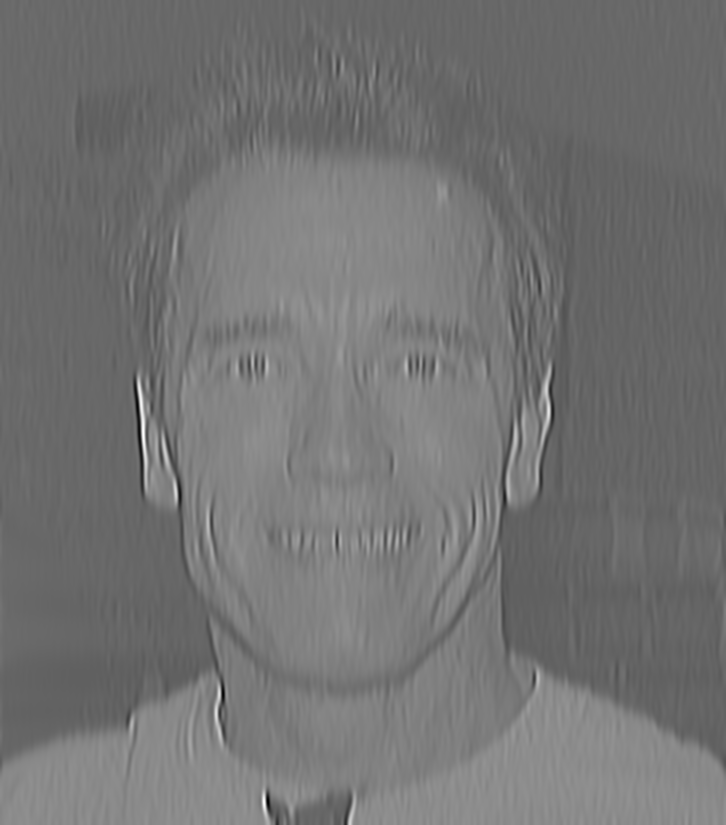
\includegraphics[width=0.5\textwidth]{./gabor/result_0.png}
\end{center} 
\subsubsection{45 degrees:}
\label{sec:orge65925c}
\begin{center}

\includegraphics[width=0.5\textwidth]{./gabor/kernel_45.png}
\end{center}
\begin{center}
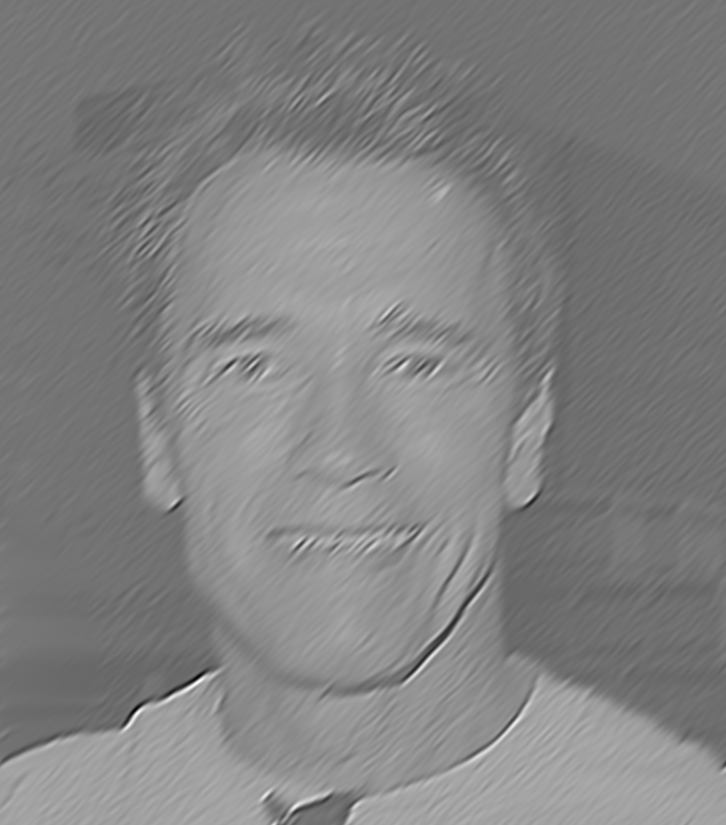
\includegraphics[width=0.5\textwidth]{./gabor/result_45.png}
\end{center}
\subsubsection{90 degrees:}
\label{sec:org154a27f}
\begin{center}

\includegraphics[width=0.5\textwidth]{./gabor/kernel_90.png}
\end{center}
\begin{center}
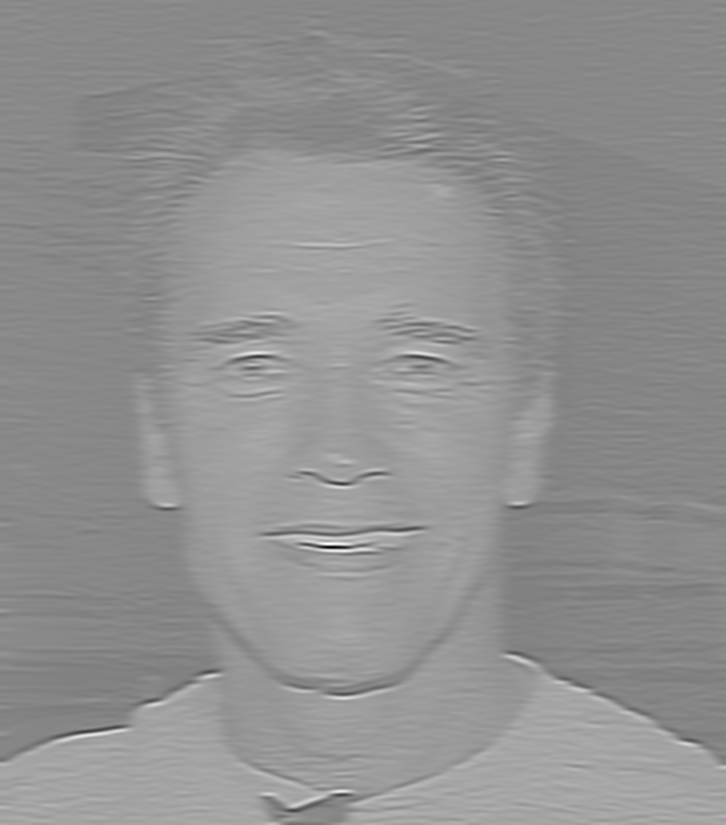
\includegraphics[width=0.5\textwidth]{./gabor/result_90.png}
\end{center}
\subsubsection{135 degrees:}
\label{sec:orgcdf0e36}
\begin{center}

\includegraphics[width=0.5\textwidth]{./gabor/kernel_135.png}
\end{center}
\begin{center}
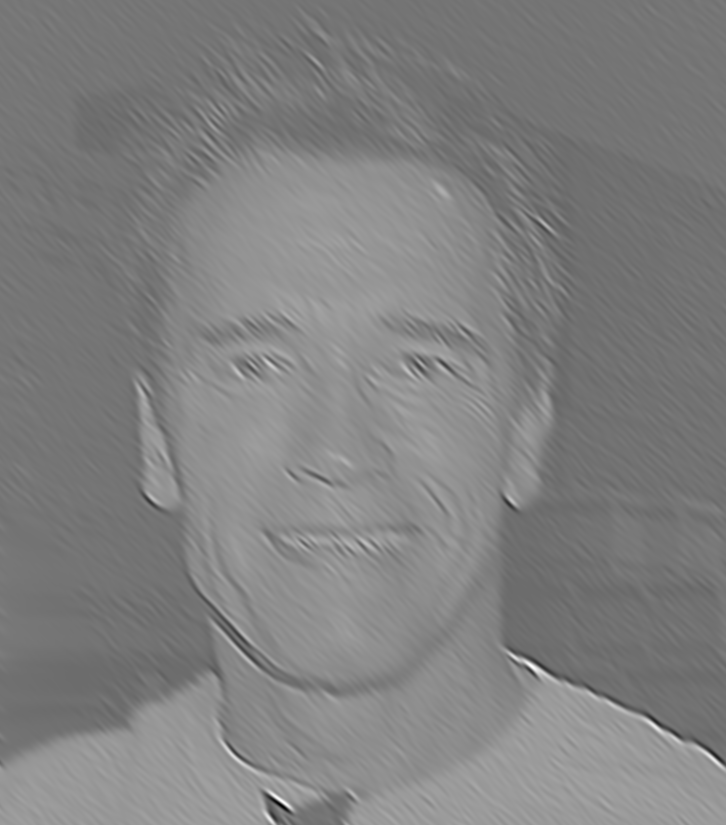
\includegraphics[width=0.5\textwidth]{./gabor/result_135.png}
\end{center}
\subsubsection{result}
\label{sec:org80f3eb9}
\begin{center}
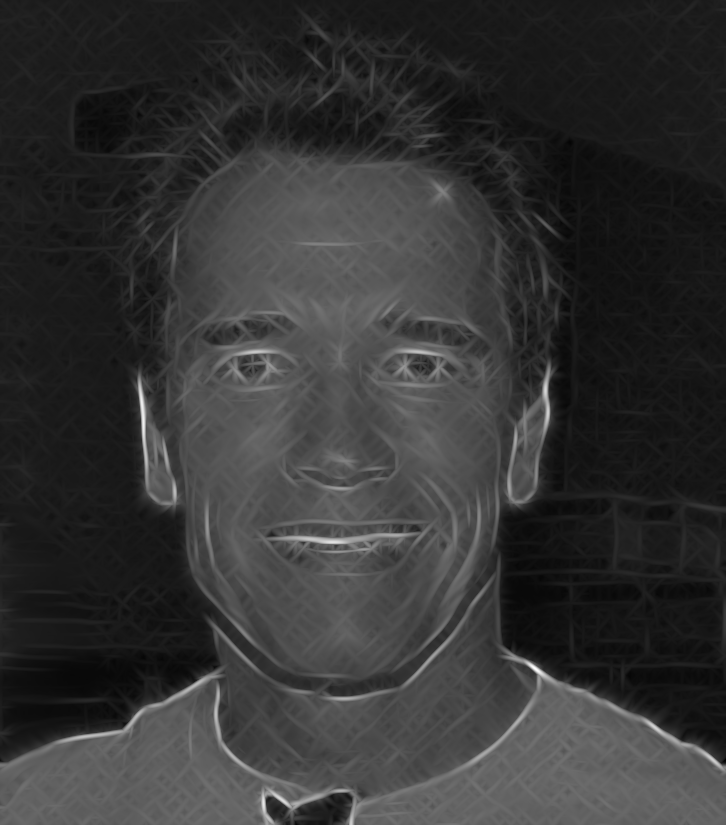
\includegraphics[width=0.5\textwidth]{./gabor/combined_max.png}
\end{center}
\subsection{playing with parameters}
\label{sec:org14fcc4a}
i use 
\begin{Code}
\begin{Verbatim}
\color{EFD}\EFk{const} \EFt{int} \EFv{ksize} = 6*sigma+1
\end{Verbatim}
\end{Code}
\subsubsection{lambda=15}
\label{sec:orgc1530a4}
\begin{center}
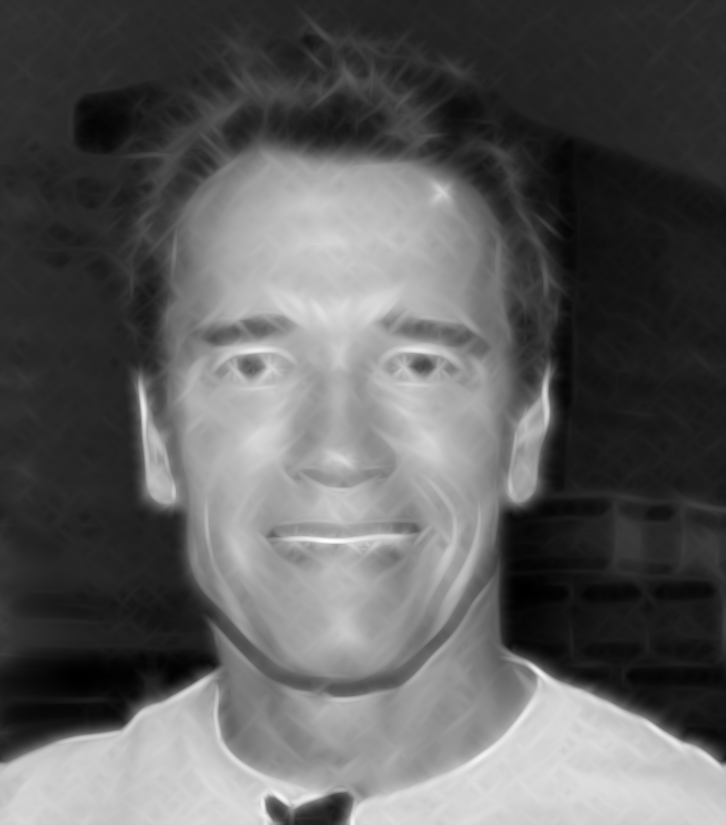
\includegraphics[width=0.5\textwidth]{./gabor/lambda_15.png}
\end{center}
\subsubsection{lambda=12}
\label{sec:org6b232f2}
\begin{center}
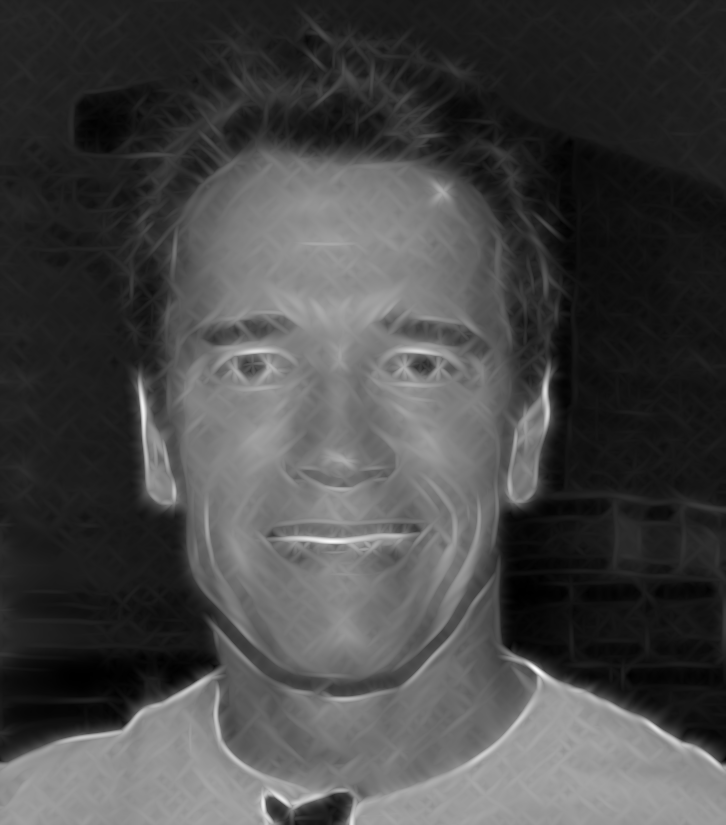
\includegraphics[width=0.5\textwidth]{./gabor/lambda_12.png}
\end{center}
\subsubsection{lambda=8}
\label{sec:orgdd1101c}
\begin{center}
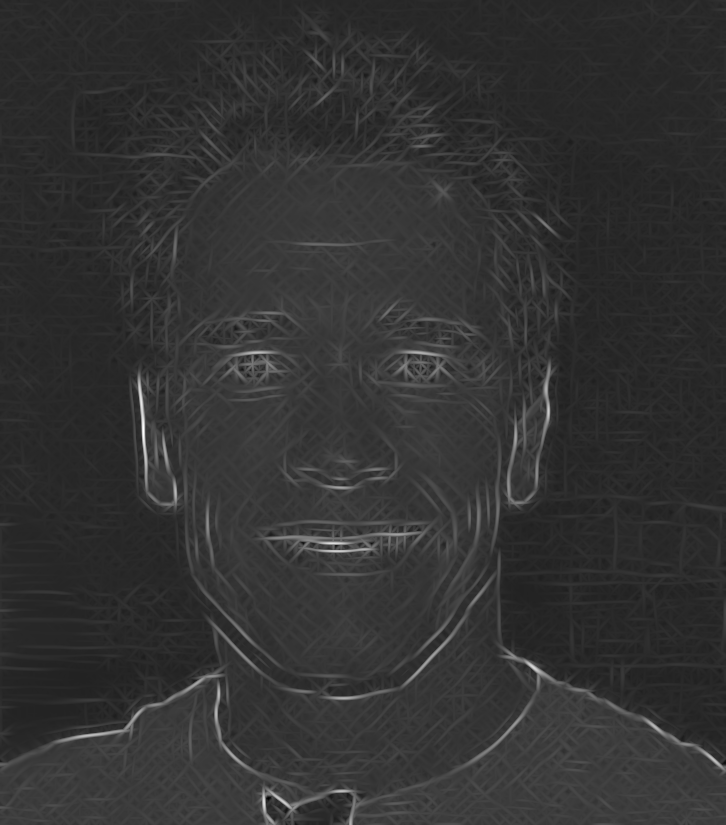
\includegraphics[width=0.5\textwidth]{./gabor/lambda_8.png}
\end{center}
\subsubsection{lambda=5}
\label{sec:org7d9c7c0}
\begin{center}
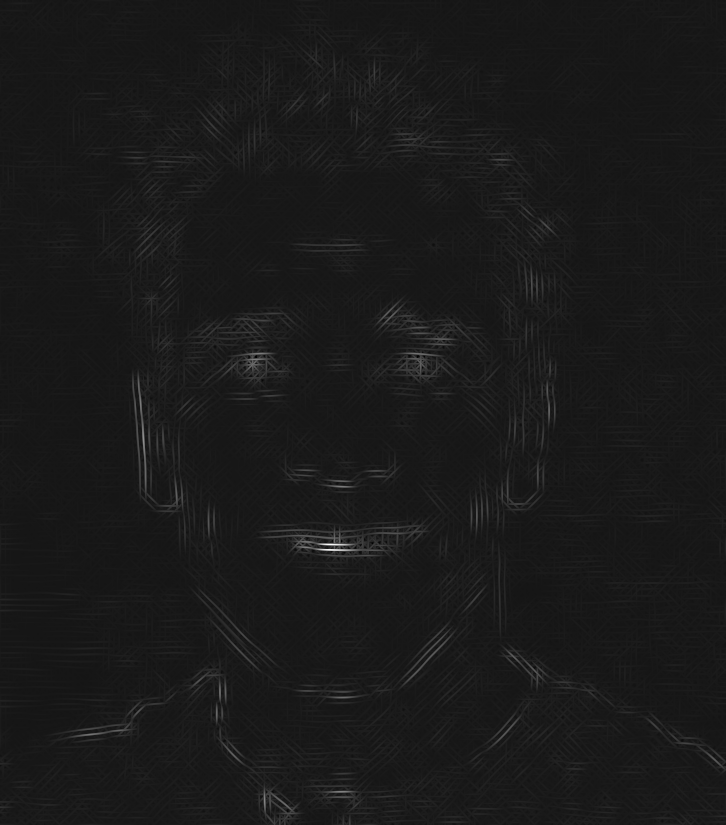
\includegraphics[width=0.5\textwidth]{./gabor/lambda_5.png}
\end{center}

For faces a lambda of around 8 seems best.
\end{document}
